\documentclass[12pt,letterpaper]{article}
\usepackage[utf8]{inputenc}
\usepackage{tikz}
\usetikzlibrary{trees}
\usepackage[spanish, es-nodecimaldot]{babel}
\usepackage{amsmath}
\usepackage{color}
\usepackage{algorithm}
\usepackage[noend]{algpseudocode}
\renewcommand{\algorithmicrequire}{\textbf{Entrada:}}
\renewcommand{\algorithmicensure}{\textbf{Salida:}}
\usepackage{subcaption}
\usepackage{amsfonts}
\usepackage{hyperref}
 \hypersetup{
     colorlinks=true,
     linkcolor=blue,
     filecolor=blue,
     citecolor = blue,      
     urlcolor=cyan,
     }
\usepackage{amssymb}
\usepackage{listings}
\usepackage{color}

\definecolor{mygreen}{rgb}{0,0.6,0}
\definecolor{mygray}{rgb}{0.5,0.5,0.5}
\definecolor{mymauve}{rgb}{0.58,0,0.82}

\lstset{ 
  backgroundcolor=\color{white},   % choose the background color; you must add \usepackage{color} or \usepackage{xcolor}; should come as last argument
  basicstyle=\footnotesize,        % the size of the fonts that are used for the code
  breakatwhitespace=false,         % sets if automatic breaks should only happen at whitespace
  breaklines=true,                 % sets automatic line breaking
  captionpos=b,                    % sets the caption-position to bottom
  commentstyle=\color{mygreen},    % comment style
  deletekeywords={...},            % if you want to delete keywords from the given language
  escapeinside={\%*}{*)},          % if you want to add LaTeX within your code
  extendedchars=true,              % lets you use non-ASCII characters; for 8-bits encodings only, does not work with UTF-8
  firstnumber=1,                % start line enumeration with line 1000
  frame=single,	                   % adds a frame around the code
  keepspaces=true,                 % keeps spaces in text, useful for keeping indentation of code (possibly needs columns=flexible)
  keywordstyle=\color{blue},       % keyword style
  language=Octave,                 % the language of the code
  morekeywords={*,...},            % if you want to add more keywords to the set
  numbers=none,                    % where to put the line-numbers; possible values are (none, left, right)
  numbersep=5pt,                   % how far the line-numbers are from the code
  numberstyle=\tiny\color{mygray}, % the style that is used for the line-numbers
  rulecolor=\color{black},         % if not set, the frame-color may be changed on line-breaks within not-black text (e.g. comments (green here))
  showspaces=false,                % show spaces everywhere adding particular underscores; it overrides 'showstringspaces'
  showstringspaces=false,          % underline spaces within strings only
  showtabs=false,                  % show tabs within strings adding particular underscores
  stepnumber=2,                    % the step between two line-numbers. If it's 1, each line will be numbered
  stringstyle=\color{mymauve},     % string literal style
  tabsize=2,	                   % sets default tabsize to 2 spaces
  title=\lstname                   % show the filename of files included with \lstinputlisting; also try caption instead of title
}

\usepackage{amsthm}
\newtheorem{theorem}{Teorema}

\usepackage{graphicx}
\usepackage[inner=1.5 cm, outer = 1.5 cm, top=1 cm, bottom = 1.5 cm]{geometry}
\setlength{\parskip}{3mm}
\title{\textsc{Práctica 7: Búsqueda local}}
\author{\textsc{Fabiola Vázquez}}

\setlength{\parindent}{0cm}
\renewcommand{\lstlistingname}{Código}
\floatname{algorithm}{Algoritmo}
\newtheorem{ej}{Ejercicio}

\begin{document}
\maketitle

\hrule
\section{Introducción}
El objetivo de esta práctica \cite{elisapractica7} es implementar una heurística para encontrar los máximos locales de la función, 
\begin{align*}
f(x,y) &= 3e^{(-(0.8y + 1)^2)-(0.8x)^2}(0.8x-1)^2 - \frac{1}{3}\cdot e^{-(0.8x+1)^2-(0.8y)^2}\\ &+e^{-(0.8x)^2-(0.8y)^2}(10(0.8x)^3-2(0.8x)+10(0.8y)^5).
\end{align*}
La figura \ref{3d} muestra la gráfica de la función $f$, pero en este tipo de gráficas es complicado la visualización de un punto moviéndose por la superficie, se opta por utilizar una representación diferente, la cual se muestra en la figura \ref{levelplot}.  El  experimento se realiza con el software R versión 4.0.2  \cite{R} en un cuaderno de Jupyter \cite{jupyter}.



\section{Experimento}
En este caso se considera el dominio de la función como $D_f = \{(x,y) \mid -3\leqslant x \leqslant 3, -3\leqslant y \leqslant 3\}$, entonces a la función $f$ se le pone la restricción de si se llega a evaluar en valores diferentes al dominio de $f$, regrese $-\infty$, esto porque se busca maximizar la función, si se busca minimizar, utilizar $\infty$.

El método utilizado para maximizar la función, consiste en posicionar un punto $(x,y)$ en el plano y dados un $\Delta x$ y un $\Delta y$ se consideran ochos vecinos, de los cuales se elige el que al evaluarlo en la función $f$ regrese el valor mayor, si ese valor es mejor que el que se tiene actualmente se considera como el nuevo mejor y se repite el proceso una cantidad \texttt{t} de iteraciones. Esto se realiza de forma automatizada con la función \texttt{replica} mostrada en el código \ref{lst:gc1}.

Se posicionan 100 puntos al azar en el plano en color negro, el mejor valor obtenido se representa con un triángulo blanco, y se realiza el proceso en 100 iteraciones, lo cual se visualiza en una \href{https://github.com/fvzqa/Simulacion/blob/master/Tarea7/Animaciones/imagen1.gif}{animación}.

Como se aprecia en la animación, en 100 pasos los cien puntos están ya atascados en algún máximo, local o global, de la función. Se realizan ahora 10,000 iteraciones, las cuales se muestran en la figura \ref{pasos}. 

\begin{lstlisting}[label=lst:gc1,caption=Función \texttt{replica}., frame = single]
replica <- function(t){ 
    currx <- runif(1, -3, 3)
    curry <- runif(1, -3, 3)
    best  <- c()
    best[1] <- currx
    best[2] <- curry
    

    for (tiempo in 1:t) {
        a <- currx
        b <- curry
        deltax <- runif(1, 0, 0.2)
        deltay <- runif(1, 0, 0.2)
        left   <- currx - deltax
        right  <- currx + deltax
        up     <- curry + deltay
        down   <- curry - deltay

        posx   <- c(left,right,a)
        posy   <- c(up,down,b)
        
        pos_max <- max(f(left,up), f(left,down),f(left,b), f(right,up), f(right,down), f(right,b), f(a,up), f(a,down))
        
        for (x in posx){
            for (y in posy){
                if(f(x,y)==pos_max){
                    currx <- x
                    curry <- y
                }
            }
        }
        
        if(f(best[1],best[2])<= f(currx,curry)){
            best[1] <- currx
            best[2] <- curry
        }
    }
    return(best)
}
    
\end{lstlisting} 

 \begin{figure}
 	\centering
 	\begin{subfigure}[b]{0.45\linewidth}
 		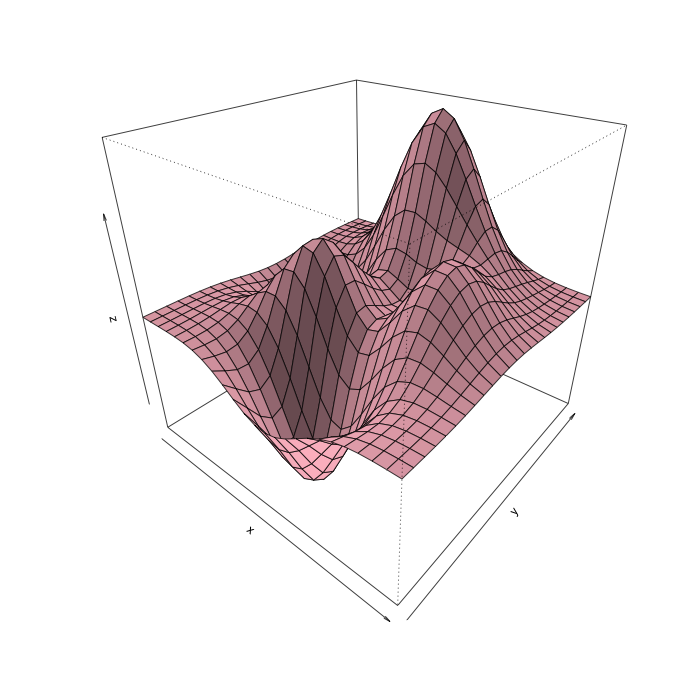
\includegraphics[width=\linewidth]{funcion_g.png}
 		 \caption{Gráfica en tres dimensiones de la función $f$.}
 		\label{3d}
 	\end{subfigure}
 	\begin{subfigure}[b]{0.45\linewidth}
 		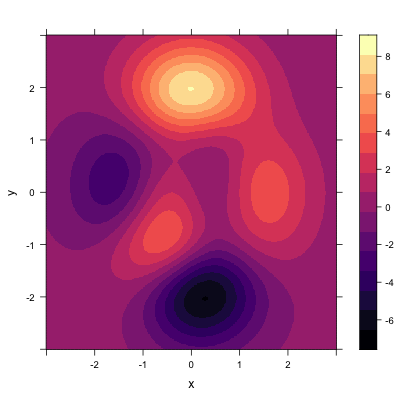
\includegraphics[width=\linewidth]{grafica.png}
 		 \caption{Gráfica de nivel de la función $f$.}
 		\label{levelplot}
 	\end{subfigure}
 	\caption{Gráficas de la función $f$.}  	
\label{graficas}
 \end{figure}
 
  \begin{figure}
 	\centering
 	\begin{subfigure}[b]{0.45\linewidth}
 		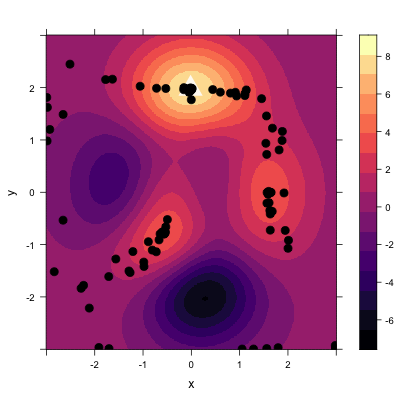
\includegraphics[width=\linewidth]{replicas_10.png}
 		 \caption{10 pasos.}
 		\label{levelplot0}
 	\end{subfigure}
 	\begin{subfigure}[b]{0.45\linewidth}
 		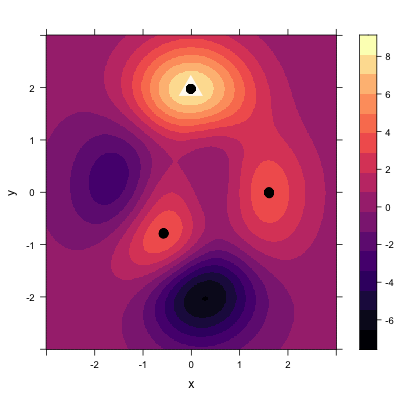
\includegraphics[width=\linewidth]{replicas_100.png}
 		 \caption{100 pasos}
 		\label{levelplot1}
 	\end{subfigure}
  	\begin{subfigure}[b]{0.45\linewidth}
 		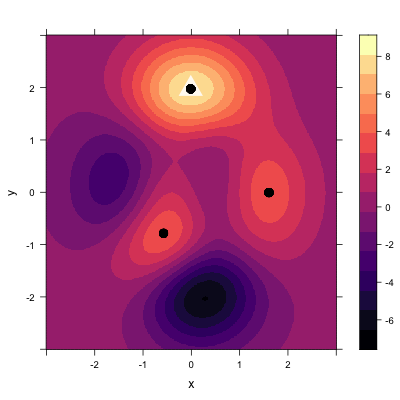
\includegraphics[width=\linewidth]{replicas_1000.png}
 		 \caption{1000 pasos.}
 		\label{levelplot1}
 	\end{subfigure}
  	\begin{subfigure}[b]{0.45\linewidth}
 		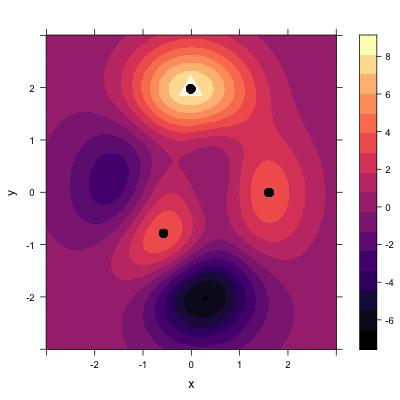
\includegraphics[width=\linewidth]{replicas_10000.png}
 		 \caption{10000 pasos.}
 		\label{levelplot2}
 	\end{subfigure}
 	\caption{Gráficas de la función $f$.}  	
\label{pasos}
 \end{figure}
 
 \section{Reto 1}
 En el reto 1, a diferencia de la tarea base, se cambia el tipo de movimiento a otro llamado \textbf{recocido simulado}, el cual compara el valor \texttt{delta} definido como la diferencia entre $f(x',y')$ y $f(x,y)$, donde $(x',y')$ es algún vecino. Si el valor de \texttt{delta} es mayor que cero, el vecino se acepta como la posición actual, ya que representa un valor mayor que el actual, pero si \texttt{delta} es menor que cero, no es una mejora, aun así se podría aceptar como vecino con una probabilidad de \texttt{exp(-delta/T)}, donde \texttt{T} es la temperatura inicial. Se tienen dos parámetros iniciales, la temperatura inicial \texttt{T} y \texttt{xi} que es la rapidez con la que \texttt{T} disminuye si se acepta un vecino que no te da un mejor valor. Al igual que en la tarea base, se realiza una \href{https://github.com/fvzqa/Simulacion/blob/master/Tarea7/Animaciones/reto1.gif}{animación} de 100 pasos ahora con este tipo de movimiento.  
 
 El objetivo es examinar los efectos estadísticos del valor inicial \texttt{T} y el valor \texttt{xi}, para ello se realiza un experimento variando dichos valores, la temperatura \texttt{T} se considera como $\{1, 10, 100, 1000, 10000\}$ y el valor de \texttt{xi} varía en $\{0.7, 0.8, 0.9, 0.95, 0.99, 0.995, 0.999 \}$.
 
 Se realiza una prueba de correlación para verificar si algún parámetro influye en si se alcanza un máximo local o no. Primero para la temperatura inicial,
 \begin{verbatim}
 Pearson's product-moment correlation

data:  datos$`Temp Inicial` and datos$max
t = 0.082459, df = 3498, p-value = 0.9343
alternative hypothesis: true correlation is not equal to 0
95 percent confidence interval:
 -0.03173876  0.03452414
sample estimates:
        cor 
0.001394216, 
 \end{verbatim}
 se tiene un valor $p \approx$ 0.93 el cual es mayor que $\alpha=0.05$, por lo que se dice que la temperatura inicial no afecta al resultado. Para el valor de \texttt{xi},
\begin{verbatim}
Pearson's product-moment correlation

data:  datos$xi and datos$max
t = 2.3218, df = 3498, p-value = 0.0203
alternative hypothesis: true correlation is not equal to 0
95 percent confidence interval:
 0.006103839 0.072265015
sample estimates:
       cor 
0.03922742, 
\end{verbatim}
se tiene un valor $p \approx 0.02$ el cual es menor que $\alpha$, por lo que se concluye que el valor de \texttt{xi} sí afecta el resultado, pero como el coeficiente de correlación \texttt{cor} $\approx$ 0.039, se concluye que sí afecta pero muy poco.  

\section{Reto 2}
En el reto 1 se llega a la conclusión de que el valor del parámetro \texttt{T} no influye en el resultado final, así que se deja fijo como \texttt{T=1}. Se realizan tres experimentos variando el valor de \texttt{xi} como 0.7,0.8 y 0.9. Para los dos métodos trabajados anteriormente, se compara el valor obtenido con el valor del máximo global, los resultados se muestran en la figura \ref{d}, donde se aprecia que los valores obtenidos con los dos métodos son similares.
  \begin{figure}
 	\centering
 	\begin{subfigure}[b]{0.5\linewidth}
 		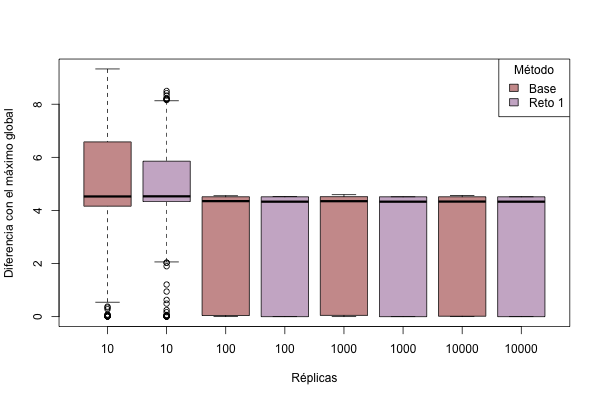
\includegraphics[width=\linewidth]{b07.png}
 		 \caption{\texttt{xi=0.7}.}
 		\label{a}
 	\end{subfigure}
 	\begin{subfigure}[b]{0.5\linewidth}
 		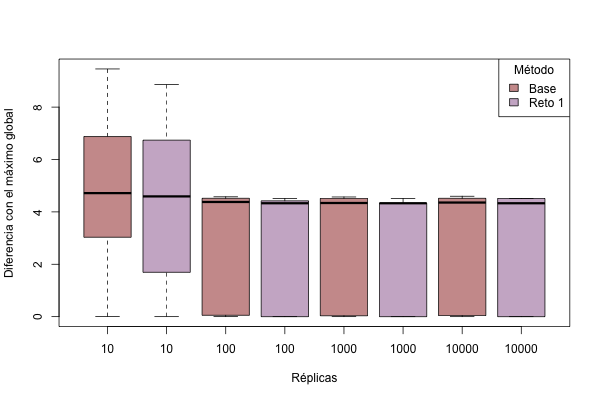
\includegraphics[width=\linewidth]{b08.png}
 		 \caption{\texttt{xi=0.8}}
 		\label{b}
 	\end{subfigure}
  	\begin{subfigure}[b]{0.5\linewidth}
 		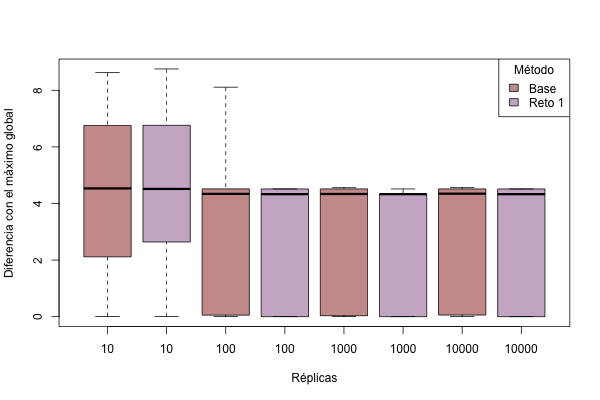
\includegraphics[width=\linewidth]{b09.png}
 		 \caption{\texttt{xi=0.9}.}
 		\label{c}
 	\end{subfigure}

 	\caption{Gráficas de caja comparando los resultados obtenidos con los métodos de la tarea base y del reto 1.}  	
\label{d}
 \end{figure}
 
Se realiza una prueba Welch para ver si hay diferencia significativa con las medias de los datos obtenidos con el método base y con el método del reto 1. 

\begin{verbatim}
Welch Two Sample t-test

data:  data$base and data$reto1
t = -1.1828, df = 794.08, p-value = 0.2372
alternative hypothesis: true difference in means is not equal to 0
95 percent confidence interval:
 -0.5212880  0.1292767
sample estimates:
mean of x mean of y 
 3.237430  3.433436 
\end{verbatim}

Dado que se obtiene un valor $p$ mayor que $0.05$, se dice que no hay diferencia significativa entre las medias de los conjuntos de datos.

\bibliographystyle{plain} 
\bibliography{Referencias}


\end{document} 